\documentclass[11pt]{article}
\usepackage[margin=1in]{geometry}
\usepackage{amsmath,amssymb}
\usepackage{booktabs}
\usepackage{graphicx}
\usepackage{siunitx}
\usepackage{hyperref}
\usepackage{natbib}
\usepackage{xcolor}
\usepackage{float}
\usepackage[capitalise]{cleveref}

\bibliographystyle{plainnat}

% S-prefix numbering for supplement
\renewcommand{\theequation}{S\arabic{equation}}
\renewcommand{\thefigure}{S\arabic{figure}}
\renewcommand{\thetable}{S\arabic{table}}

\title{Supplementary Materials\\[2mm]
\large Energy-efficient codon optimization on thermodynamic hardware}

\author{
Andraž Jelinčič,$^{1,}$\footnote{Corresponding author: \texttt{andraz@extropic.ai}} \hspace{5mm} Ross C.\ Walker$^{1}$ \\[2mm]
\small $^{1}$Extropic Corp., Boston, MA
}

\date{}

\begin{document}
\maketitle

% ============================================================
% SUPPLEMENTARY NOTE 1
% ============================================================
\section*{Supplementary Note 1: Domain-wall encoding derivation}

This note provides the full mathematical derivation of how Potts model weights are compiled to Ising model weights via domain-wall encoding (DWE)~\cite{chancellor2019dwc, berwald2022dwc}, as referenced in Section~4.4 of the main text.

\subsection*{Setup and notation}

Consider a single Potts variable $c \in \{0, 1, \ldots, K{-}1\}$ with energy $E(c) = h_c$ for each state.
We seek an Ising model on $\{-1,+1\}$ spins that reproduces these energies exactly (up to a constant) on valid configurations and penalizes invalid ones.

\subsection*{Thermometer encoding and constraint}

Introduce $K{-}1$ Ising spins $s_1, \ldots, s_{K-1} \in \{-1,+1\}$.
Potts state $k$ is encoded as the ``thermometer'' pattern~\cite{chancellor2019dwc} where the first $k$ spins are $+1$ and the rest are $-1$:
\begin{equation}\label{eq:thermo}
  c = k \quad\Longleftrightarrow\quad
  s_i = \begin{cases} +1 & i \leq k \\ -1 & i > k \end{cases}
\end{equation}
The ``domain wall''---the boundary between the $+1$ and $-1$ regions---sits at position $k$.

Invalid configurations (those with a $-1$ followed by a $+1$, i.e.\ a reverse domain wall) are penalized.
In $\{0,1\}$ variables $q_i = (1+s_i)/2$, the penalty for a single reverse wall between positions $i$ and $i{+}1$ is $P \cdot q_{i+1}(1 - q_i)$.
Converting to $\{-1,+1\}$ spins:
\begin{equation}\label{eq:constraint}
  H_{\mathrm{constr}} = \frac{P}{4} \sum_{i=1}^{K-2} \bigl(1 - s_i + s_{i+1} - s_i s_{i+1}\bigr)
\end{equation}
This equals zero on all valid (thermometer) configurations and adds $P$ for each reverse domain wall.
The constraint graph is a \emph{chain} ($K{-}2$ edges), which is 2-colorable---in contrast to the $K(K{-}1)/2$-edge clique required by one-hot encoding~\cite{lucas2014ising}.

\subsection*{Single-variable Ising Hamiltonian}

The indicator for Potts state $k$ can be written as $\delta_{c=k} = q_k - q_{k+1}$ (defining $q_0 \equiv 1$, $q_K \equiv 0$).
Therefore $\sum_k h_k\,\delta_{c=k} = h_0 + \sum_{i=1}^{K-1}(h_i - h_{i-1})\,q_i$.
Converting to $\{-1,+1\}$ spins:
\begin{equation}\label{eq:bias}
  H_{\mathrm{bias}} = \sum_{i=1}^{K-1} \frac{h_i - h_{i-1}}{2}\, s_i + \mathrm{const}
\end{equation}

Combining \cref{eq:constraint} and \cref{eq:bias} and collecting terms:
\begin{equation}\label{eq:single-full}
\boxed{
  H = \sum_{i=1}^{K-1} b_i\, s_i \;-\; \frac{P}{4}\sum_{i=1}^{K-2} s_i\, s_{i+1} \;+\; \mathrm{const}
}
\end{equation}
where the local fields are:
\begin{equation}\label{eq:fields}
  b_i = \frac{h_i - h_{i-1}}{2} +
  \begin{cases}
    -P/4 & i = 1 \\
    0 & 2 \leq i \leq K{-}2 \\
    +P/4 & i = K{-}1
  \end{cases}
\end{equation}
The couplings $J_{i,i+1} = -P/4$ are \textbf{ferromagnetic} (favoring aligned spins), forming a nearest-neighbor chain.

\subsection*{Worked example: $K=4$}

Consider Potts biases $h_0, h_1, h_2, h_3$.
Three Ising spins $s_1, s_2, s_3$ yield the Hamiltonian:
\begin{equation}
  H = b_1\, s_1 + b_2\, s_2 + b_3\, s_3 - \tfrac{P}{4}\, s_1 s_2 - \tfrac{P}{4}\, s_2 s_3 + \mathrm{const}
\end{equation}
with
\begin{equation}
  b_1 = \frac{h_1 - h_0}{2} - \frac{P}{4}, \qquad
  b_2 = \frac{h_2 - h_1}{2}, \qquad
  b_3 = \frac{h_3 - h_2}{2} + \frac{P}{4}
\end{equation}

\subsection*{Multi-variable case: pairwise interactions}

Consider $L$ Potts variables $c_1, \ldots, c_L$ with unary biases $h^{(p)}_k$ and pairwise interactions $V^{(pq)}_{kl}$~\cite{chancellor2019dwc, berwald2022dwc}:
\begin{equation}\label{eq:potts-energy}
  E = \sum_p \sum_k h^{(p)}_k \,\delta_{c_p=k}
    \;+\; \sum_{(p,q)} \sum_{k,l} V^{(pq)}_{kl}\,\delta_{c_p=k}\,\delta_{c_q=l}
\end{equation}
Each position $p$ gets its own domain-wall chain of $K_p{-}1$ spins $s_{p,1},\ldots,s_{p,K_p-1}$.
The unary terms convert exactly as before (\cref{eq:bias,eq:fields}).
Below we derive how pairwise Potts interactions compile to Ising couplings.

\paragraph{Step 1: Abel summation in $\{0,1\}$ variables.}

Using the indicator identity $\delta_{c_p=k} = q_{p,k} - q_{p,k+1}$ (with $q_{p,0}\equiv 1$, $q_{p,K_p}\equiv 0$) and the standard Abel summation formula
$\sum_{k=0}^{K-1} f_k\,(q_k - q_{k+1}) = f_0 + \sum_{i=1}^{K-1}(f_i - f_{i-1})\,q_i$,
we expand the pairwise energy between positions $p$ and $q$.

First, sum over $l$ for fixed $k$:
\begin{equation}
  \sum_l V_{kl}\,(q_{q,l} - q_{q,l+1})
  = V_{k,0} + \sum_{j=1}^{K_q-1}(V_{k,j} - V_{k,j-1})\,q_{q,j}
\end{equation}
Then sum over $k$, applying Abel summation to each coefficient separately:
\begin{equation}\label{eq:abel-result}
  E_{pq}
  = V_{0,0}
    + \sum_{i=1}^{K_p-1} \alpha_i\, q_{p,i}
    + \sum_{j=1}^{K_q-1} \beta_j\, q_{q,j}
    + \sum_{i=1}^{K_p-1}\sum_{j=1}^{K_q-1} \widetilde{V}_{ij}\, q_{p,i}\, q_{q,j}
\end{equation}
where
\begin{align}
  \alpha_i &= V_{i,0} - V_{i-1,0}
    & &\text{(first difference along column $l{=}0$)} \label{eq:alpha}\\
  \beta_j &= V_{0,j} - V_{0,j-1}
    & &\text{(first difference along row $k{=}0$)} \label{eq:beta}\\[4pt]
  \widetilde{V}_{ij} &= V_{ij} - V_{i-1,j} - V_{i,j-1} + V_{i-1,j-1}
    & &\text{(mixed second difference)} \label{eq:mixed-diff}
\end{align}

\paragraph{Step 2: convert to $\{-1,+1\}$ spins.}

Substitute $q_{p,i} = (1+s_{p,i})/2$ into \cref{eq:abel-result}.
The linear and quadratic terms expand as:
\begin{align}
  \alpha_i\, q_{p,i} &= \tfrac{\alpha_i}{2} + \tfrac{\alpha_i}{2}\, s_{p,i} \\[2pt]
  \widetilde{V}_{ij}\, q_{p,i}\, q_{q,j}
    &= \tfrac{\widetilde{V}_{ij}}{4}
     + \tfrac{\widetilde{V}_{ij}}{4}\, s_{p,i}
     + \tfrac{\widetilde{V}_{ij}}{4}\, s_{q,j}
     + \tfrac{\widetilde{V}_{ij}}{4}\, s_{p,i}\, s_{q,j}
\end{align}
Collecting all terms by type yields:

\paragraph{Inter-position couplings.}
\begin{equation}\label{eq:Jinter}
\boxed{\;
  J^{\mathrm{inter}}_{(p,i),(q,j)} = \frac{\widetilde{V}_{ij}}{4}
  = \frac{V_{ij} - V_{i-1,j} - V_{i,j-1} + V_{i-1,j-1}}{4}
\;}
\end{equation}

\paragraph{Bias contributions from pairwise interactions.}
Each pairwise interaction $(p,q)$ contributes an additional bias to spins at both positions.
For spin $s_{p,i}$:
\begin{equation}\label{eq:bias-pairwise}
  b_{p,i}^{(pq)}
  = \frac{\alpha_i}{2} + \frac{1}{4}\sum_{j=1}^{K_q-1} \widetilde{V}_{ij}
  = \frac{(V_{i,0} - V_{i-1,0}) + (V_{i,K_q-1} - V_{i-1,K_q-1})}{4}
\end{equation}
where the simplification uses the fact that $\sum_j \widetilde{V}_{ij}$ telescopes.
Symmetrically, for spin $s_{q,j}$:
\begin{equation}\label{eq:bias-pairwise-q}
  b_{q,j}^{(pq)}
  = \frac{(V_{0,j} - V_{0,j-1}) + (V_{K_p-1,j} - V_{K_p-1,j-1})}{4}
\end{equation}

\paragraph{Complete multi-position Ising Hamiltonian.}
Combining unary terms (\cref{eq:fields}), constraint chains (\cref{eq:constraint}), and pairwise terms (\cref{eq:Jinter,eq:bias-pairwise,eq:bias-pairwise-q}):
\begin{equation}\label{eq:full-multi}
\boxed{
  H = \sum_p \sum_{i=1}^{K_p-1} b_{p,i}\, s_{p,i}
    \;-\; \frac{P}{4}\sum_p \sum_{i=1}^{K_p-2} s_{p,i}\, s_{p,i+1}
    \;+\; \sum_{(p,q)} \sum_{i,j} \frac{\widetilde{V}^{(pq)}_{ij}}{4}\, s_{p,i}\, s_{q,j}
    \;+\; \mathrm{const}
}
\end{equation}
The total bias on spin $s_{p,i}$ is:
\begin{equation}\label{eq:total-bias}
  b_{p,i} = \underbrace{\frac{h^{(p)}_i - h^{(p)}_{i-1}}{2}}_{\text{Potts unary}}
  + \underbrace{\text{boundary}_{P}(i)}_{\text{constraint}}
  + \underbrace{\sum_{q:\,(p,q)\in\mathcal{E}} b_{p,i}^{(pq)}}_{\text{pairwise (\cref{eq:bias-pairwise})}}
\end{equation}
where $\text{boundary}_P(i) = -P/4$ if $i=1$, $+P/4$ if $i=K_p{-}1$, and $0$ otherwise.

The Ising model has two types of edges:
\begin{itemize}
  \item \textbf{Constraint chains} (coupling $-P/4$, ferromagnetic): $s_{p,i}\leftrightarrow s_{p,i+1}$ within each position.
  \item \textbf{Inter-position couplings} (coupling $\widetilde{V}_{ij}/4$): $s_{p,i}\leftrightarrow s_{q,j}$ for each pair of interacting Potts positions, with $(K_p{-}1)(K_q{-}1)$ such couplings per Potts edge.
\end{itemize}

\subsection*{P-independent mixing at the domain wall}

A Gibbs update at the domain wall boundary---where spin $s_i$ has neighbor $s_{i-1} = +1$ (inside the wall) and $s_{i+1} = -1$ (outside)---sees an effective field:
\begin{equation}
  h_{\mathrm{eff}} = b_i + J \cdot s_{i-1} + J \cdot s_{i+1} = b_i + J \cdot (+1) + J \cdot (-1) = b_i
\end{equation}
The two ferromagnetic coupling contributions cancel exactly.
The domain wall therefore performs a random walk governed only by the bias landscape $\{b_i\}$, completely independent of the penalty strength $P$.

This is the key advantage of DWE over one-hot encoding.
In one-hot encoding, the penalty clique creates genuine energy barriers that scale with $P$, leading to exponentially slow mixing at large $P$~\cite{berwald2022dwc, levin2009markov}.
In DWE, the constraint can be made arbitrarily strong without affecting the sampling dynamics at the domain wall.

\subsection*{4-color block decomposition}

The Ising graph for the codon problem is 4-colorable using the coloring $(p_{\mathrm{parity}},\, j_{\mathrm{parity}})$, where $p_{\mathrm{parity}} = p \bmod 2$ is the position parity and $j_{\mathrm{parity}} = j \bmod 2$ is the spin-index parity within each position's chain.
The key observation is that constraint edges connect spins within the same position (same $p_{\mathrm{parity}}$, different $j_{\mathrm{parity}}$), while inter-position edges connect spins at adjacent positions (different $p_{\mathrm{parity}}$).
Therefore, no two spins sharing the same $(p_{\mathrm{parity}},\, j_{\mathrm{parity}})$ pair are connected by an edge, and each of the four color classes can be updated simultaneously in a parallel Gibbs step.

\subsection*{Comparison of encoding schemes}

\Cref{tab:encodings} summarizes the key properties of three encoding schemes for mapping a $K$-state Potts variable to binary spins.

\begin{table}[H]
\centering
\caption{Comparison of encoding schemes for a $K$-state Potts variable. Values in parentheses are for $K=6$ (the maximum in the codon problem).}
\label{tab:encodings}
\vspace{2mm}
\begin{tabular}{lcccc}
\toprule
Property & Native Potts & One-hot & Domain wall & Binary \\
\midrule
Variables & 1 categorical & $K$ (6) & $K{-}1$ (5) & $\lceil\log_2 K\rceil$ (3) \\
Constraint edges & 0 & $\frac{K(K{-}1)}{2}$ (15) & $K{-}2$ (4) & complex \\
Penalty strength & N/A & large & ${\sim}2$--$5\times$ smaller & complex \\
Chromatic impact & none & $\geq K$-fold & none (2-colorable) & unpredictable \\
Gibbs mixing & optimal & poor at large $P$ & $P$-independent & very poor \\
\bottomrule
\end{tabular}
\end{table}

Domain-wall encoding offers several advantages over one-hot encoding~\cite{chancellor2019dwc, berwald2022dwc, chen2021dwc}.
The constraint graph is a chain rather than a clique, yielding a much sparser graph and lower penalty requirements.
The chain constraint is 2-colorable, so it at most doubles the chromatic number of the overall graph---unlike one-hot, which can increase it $K$-fold.
DWE has been proven optimal in the number of binary variables for quadratic interactions~\cite{berwald2022dwc}.
Finally, Chen et al.~\cite{chen2021dwc} demonstrated experimentally that DWE outperforms one-hot encoding, with a D-Wave 2000Q using DWE outperforming the next-generation D-Wave Advantage with one-hot encoding.
Binary encoding uses the fewest variables ($\lceil\log_2 K\rceil$) but introduces complex, non-local constraint structures that are difficult to enforce and lead to poor mixing.

% ============================================================
% SUPPLEMENTARY NOTE 2
% ============================================================
\section*{Supplementary Note 2: Energy estimation details}

This note provides the detailed methodology for the energy estimates presented in Section~4.7 of the main text.

\subsection*{TSU energy model (Ising chip)}

We use the energy model from Jelincic et al.~\cite{jelincic2025dtm} (Appendix~E), which provides a physical model of an all-transistor Boltzmann machine Gibbs sampler.
The total energy for a sampling run is:
\begin{equation}\label{eq:ising-energy}
  E = n_{\mathrm{iter}} \times N \times E_{\mathrm{cell}}
\end{equation}
where $n_{\mathrm{iter}}$ is the number of Gibbs iterations, $N$ is the number of spins, and $E_{\mathrm{cell}} \approx 1.3$~fJ is the energy per spin per Gibbs step.

The per-cell energy $E_{\mathrm{cell}}$ breaks down into four components:
\begin{itemize}
  \item $E_{\mathrm{rng}} \approx 350$~aJ: energy consumed by the all-transistor random number generator, based on direct measurements from a prototype chip. The RNG exploits shot-noise dynamics of subthreshold transistors and has a decorrelation time of ${\sim}100$~ns.
  \item $E_{\mathrm{bias}}$: energy consumed by the biasing circuitry (a linear resistor network that computes a biasing voltage from neighbor states).
  \item $E_{\mathrm{clock}}$: energy consumed by clocking circuitry that orchestrates the sequential color-block updates.
  \item $E_{\mathrm{comm}}$: energy consumed by inter-cell communication (charging wires to neighboring cells).
\end{itemize}

This model captures all central functional units of a hardware Boltzmann machine sampler.
When comparing the results of this type of calculation to a detailed analysis of a complete device design (Cadence simulations), agreement is found within an order of magnitude~\cite{jelincic2025dtm}.

For the codon optimization problem, the Ising model has $N = 3{,}147$ spins with a maximum degree of 12 and only local connectivity, closely matching the setup analyzed in~\cite{jelincic2025dtm}.
With $n_{\mathrm{iter}} = 2 \times 10^4$ Gibbs iterations:
\begin{equation}
  E_{\mathrm{Ising}} = 2 \times 10^4 \times 3{,}147 \times 1.3 \times 10^{-15}~\text{J} \approx 82~\text{nJ}
\end{equation}

\subsection*{TSU energy model (Potts chip, projected)}

The Potts chip energy estimate is based on a physical model of a p-dit (categorical) sampling circuit, extrapolated from prototype measurements of p-bit circuits.
The key energy-consuming components are:

\begin{itemize}
  \item \textbf{P-bit sampling}: each p-cell draws ${\sim}800$~aJ per random sample from its internal stochastic circuit.
  \item \textbf{MACDAC} (multiply-accumulate DAC): computes the conditional bias for each Potts state from neighbor states. For a node with $q$ states and $d$ neighbors, the MACDAC has $d \cdot \lceil\log_2 q\rceil + 2$ inputs, with an output capacitance of ${\sim}500$~aF per input.
  \item \textbf{Communication}: wires carrying state information to neighboring cells, with capacitance ${\sim}350$~aF/$\mu$m.
  \item \textbf{Clocking}: global clock distribution for coordinating block updates.
\end{itemize}

Each p-cell requires ${\sim}q \times 10$ relaxation steps for its internal Markov chain (where $q$ is the number of Potts states), yielding a total energy of ${\sim}0.084$~nJ per Gibbs sweep for $L = 1{,}273$ Potts nodes.
Over 10 sweeps: $10 \times 0.084 \approx 0.84$~nJ.

We note that Potts (p-dit) hardware does not yet exist; only the Ising (p-bit) TSU is the near-term target.
For an example of how a Potts model could be implemented in CMOS hardware, see Whitehead et al.~\cite{whitehead2023}.

\subsection*{GPU FLOP counting}

\Cref{tab:flops} summarizes the FLOP estimates for each algorithm.
These are order-of-magnitude estimates; the key observation is that the algorithms span several orders of magnitude in computational cost for comparable solution quality.

\begin{table}[H]
\centering
\caption{FLOP estimates for each optimization algorithm on the spike protein ($L = 1{,}273$).}
\label{tab:flops}
\vspace{2mm}
\begin{tabular}{llrr}
\toprule
Algorithm & Per-step cost & Steps & Total FLOPs \\
\midrule
Potts (10 sweeps) & ${\sim}100$ FLOPs/position & $10 \times 1{,}273$ & ${\sim}1.3 \times 10^6$ \\
Ising ($2 \times 10^4$ sweeps) & ${\sim}32$ FLOPs/spin & $2 \times 10^4 \times 3{,}147$ & ${\sim}2.0 \times 10^9$ \\
GA (tuned) & see below & $200 \times 1{,}000$ & ${\sim}6 \times 10^9$ \\
\bottomrule
\end{tabular}
\end{table}

\paragraph{Potts model (${\sim}1.3 \times 10^6$ FLOPs).}
Each of the 10 Gibbs sweeps updates all $L = 1{,}273$ positions.
Per position, the computation involves: bias lookup ($K = 6$ values), two neighbor interaction lookups (indexing into a $K \times K$ pairwise matrix), softmax normalization over $K$ states (${\sim}3K$ operations for exponentiation and normalization), and a categorical sample (${\sim}K$ operations for cumulative sum and comparison).
This totals ${\sim}100$ FLOPs per position.

\paragraph{Ising model (${\sim}2.0 \times 10^9$ FLOPs).}
Each of the $2 \times 10^4$ Gibbs sweeps updates all $N = 3{,}147$ spins.
Per spin: computing the effective field from ${\sim}12$ neighbors requires ${\sim}24$ multiply-add operations, plus the bias term (1 operation), a sigmoid evaluation (${\sim}5$ operations for the approximation), and a Bernoulli sample (2 operations).
This totals ${\sim}32$ FLOPs per spin.

\paragraph{Genetic algorithm (${\sim}6 \times 10^9$ FLOPs).}
With population size 200 and $1{,}000$ generations, each generation involves:
\begin{itemize}
  \item \textit{Scoring} (${\sim}6L$ FLOPs per individual): GC counting (sum over $L$ positions), repeat penalty lookup ($L{-}1$ table lookups and additions), and rarity score lookup ($L$ table lookups).
  \item \textit{Crossover} (${\sim}5L$ FLOPs per offspring): parent selection (random index), uniform crossover mask generation and application.
  \item \textit{Mutation} (${\sim}15L$ FLOPs per offspring): for each position, generate a random number, compare against mutation rate, and when mutating, perform frequency-weighted codon sampling (cumulative probability lookup).
  \item \textit{Selection and sorting}: ranking the population by score.
\end{itemize}
The GA requires ${\sim}5{,}000\times$ more FLOPs than the Potts sampler for comparable solution quality.

\subsection*{GPU energy bounds}

We estimate GPU energy on an NVIDIA RTX~3090 (350~W TDP, 35.6~TFLOPS FP32 peak) using two methods:

\paragraph{Idealized lower bound.}
The idealized energy is computed as:
\begin{equation}
  E_{\mathrm{ideal}} = \frac{\text{Total FLOPs}}{\text{Peak FLOP/s}} \times \text{TDP}
  = \frac{\text{Total FLOPs}}{35.6 \times 10^{12}} \times 350~\text{W}
\end{equation}
This is a generous lower bound: no real workload sustains 100\% utilization, and the codon optimization workloads are far too small to saturate a modern GPU.

\paragraph{Measured upper bound.}
The measured energy multiplies the wall-clock execution time of our JIT-compiled JAX implementation by TDP:
\begin{equation}
  E_{\mathrm{measured}} = t_{\mathrm{wall}} \times 350~\text{W}
\end{equation}
This is an upper bound since the GPU may not draw full TDP power during execution.

\Cref{tab:gpu-energy} summarizes both estimates.
The large gap between idealized and measured energy (2--4 orders of magnitude for the Potts model) reflects the fact that these workloads are too small to efficiently utilize GPU hardware: execution time is dominated by kernel launch overhead, memory latency, and pipeline stalls rather than by floating-point computation.

\begin{table}[H]
\centering
\caption{GPU energy estimates on an NVIDIA RTX~3090 (350~W TDP, 35.6~TFLOPS FP32 peak). The Ising wall time was estimated by scaling from an RTX 4080 Laptop measurement.}
\label{tab:gpu-energy}
\vspace{2mm}
\begin{tabular}{lrrrr}
\toprule
Algorithm & FLOPs & Idealized energy & Wall time & Measured energy \\
\midrule
Potts (10 sweeps) & $1.3 \times 10^6$ & 13~\textmu J & 0.7~ms & 245~mJ \\
Ising ($2 \times 10^4$ sweeps) & $2.0 \times 10^9$ & 20~mJ & ${\sim}240$~ms & ${\sim}84$~J \\
GA (tuned) & $6 \times 10^9$ & 58~mJ & 60~ms & 21~J \\
\bottomrule
\end{tabular}
\end{table}

% ============================================================
% SUPPLEMENTARY NOTE 3
% ============================================================
\section*{Supplementary Note 3: Algorithm details and hyperparameters}

This note provides full hyperparameter tables and algorithmic details for reproducibility.

\subsection*{Hyperparameter tables}

\Cref{tab:potts-params,tab:ising-params,tab:ga-params} list all parameters used for the results reported in the main text.

\begin{table}[H]
\centering
\caption{Potts model hyperparameters.}
\label{tab:potts-params}
\vspace{2mm}
\begin{tabular}{ll}
\toprule
Parameter & Value \\
\midrule
Sequence & SARS-CoV-2 spike protein ($L = 1{,}273$) \\
Host organism & \emph{E. coli} K-12 \\
Codon usage weight $w_f$ & 0.1 \\
GC content weight $w_{\mathrm{GC}}$ & 1.0 (standard) / $2 \times 10^4$ (hard) \\
Repeat penalty weight $w_R$ & 0.1 (standard) / 0.2 (hard) \\
Target GC fraction $\rho_T$ & 0.5 \\
Number of Potts states $K_{\mathrm{max}}$ & 6 (padded) \\
Annealing steps $T$ & 10 \\
$\beta_{\mathrm{min}}$ & 0.3 \\
$\beta_{\mathrm{max}}$ & 100 \\
Gibbs sweeps per step & 1 \\
Total Gibbs sweeps & 10 \\
Adaptive GC multiplier $\eta$ & 1.0 \\
Block decomposition & 2-color (even/odd positions) \\
Independent chains & 512 \\
\bottomrule
\end{tabular}
\end{table}

\begin{table}[H]
\centering
\caption{Ising model hyperparameters.}
\label{tab:ising-params}
\vspace{2mm}
\begin{tabular}{ll}
\toprule
Parameter & Value \\
\midrule
Energy function weights & Same as Potts (\cref{tab:potts-params}) \\
Total spins $N$ & 3{,}147 \\
Average spins per position & 2.47 \\
Maximum node degree & 12 \\
Annealing steps $T$ & 10 \\
Sweeps per step & 2{,}000 (standard) / 4{,}000 (hard) \\
Total Gibbs sweeps & $2 \times 10^4$ (standard) / $4 \times 10^4$ (hard) \\
$\beta_{\mathrm{min}}$, $\beta_{\mathrm{max}}$ & 2.0, 200 (standard) / 0.5, 150 (hard) \\
$P_{\mathrm{min}}$, $P_{\mathrm{max}}$ & 2.0, 200 (standard) / 4.0, 150 (hard) \\
Initial constant-$P$ steps $n_{\mathrm{const}}$ & 5 \\
Adaptive GC multiplier & 0.9 \\
Block decomposition & 4-color (position parity $\times$ spin-index parity) \\
Independent chains & 512 \\
\bottomrule
\end{tabular}
\end{table}

\begin{table}[H]
\centering
\caption{Genetic algorithm hyperparameters.}
\label{tab:ga-params}
\vspace{2mm}
\begin{tabular}{ll}
\toprule
Parameter & Value \\
\midrule
Population size & 200 \\
Generations & 1{,}000 \\
Elite survivors & 10 \\
Lucky survivors (random) & 2 \\
Mutation rate & 0.003 \\
Crossover type & Uniform \\
Initialization & Frequency-weighted random sampling \\
Independent chains & 512 \\
\bottomrule
\end{tabular}
\end{table}

\subsection*{GA parameter sensitivity}

The genetic algorithm's performance is highly sensitive to the mutation rate.
The default mutation rate of $0.05$ from Fox et al.~\cite{fox2021mrna} yields scores in the range ${\sim}550$--$600$ on the spike protein under the hard parameter setting, and comparably degraded performance under the standard weights.
Reducing the mutation rate to $0.003$ is required to achieve scores comparable to the Potts and Ising models under both parameter settings.

This sensitivity has a natural interpretation: the uniform crossover operator already provides substantial exploration by recombining partial solutions from different individuals.
A high mutation rate is counterproductive because it disrupts good partial solutions faster than selection can preserve them.
The optimal mutation rate balances the need to introduce novel codon choices (which crossover alone cannot produce) against the cost of destroying beneficial codon combinations that selection has accumulated.

We identified the optimal parameters through a systematic sweep over mutation rate ($0.001$--$0.1$), population size ($50$--$500$), and number of elite survivors ($5$--$20$), evaluating each configuration over multiple seeds.

\subsection*{Annealing schedules}

Both the Potts and Ising models use simulated annealing~\cite{kirkpatrick1983sa} with a log-spaced inverse temperature schedule:
\begin{equation}\label{eq:beta-schedule}
  \beta_t = \beta_{\mathrm{min}} \cdot \left( \frac{\beta_{\mathrm{max}}}{\beta_{\mathrm{min}}} \right)^{t/T}
\end{equation}
for $t \in \{0, \ldots, T\}$, where $T$ is the number of annealing steps.
At each step, the host updates $\beta$, recomputes the adaptive GC coefficient, and runs a fixed number of Gibbs sweeps.

For the Ising model, the constraint penalty $P$ follows an independent schedule: it stays constant at $P_{\mathrm{min}}$ for the first $n_{\mathrm{const}}$ steps, then ramps logarithmically:
\begin{equation}\label{eq:P-schedule}
  P_t = \begin{cases}
    P_{\mathrm{min}} & t \leq n_{\mathrm{const}} \\[4pt]
    P_{\mathrm{min}} \cdot \left( \dfrac{P_{\mathrm{max}}}{P_{\mathrm{min}}} \right)^{(t - n_{\mathrm{const}})/(T - n_{\mathrm{const}})} & t > n_{\mathrm{const}}
  \end{cases}
\end{equation}
Low $P$ early in annealing permits invalid-state (defect) transitions that provide shortcuts around energy barriers: when a valid intermediate state $k$ has energy exceeding $P$, the defect route (costing $P$) is energetically cheaper.
High $P$ at the end enforces strict constraint satisfaction.

\subsection*{Spike protein spin count}

The spike protein ($L = 1{,}273$) maps to $N = 3{,}147$ domain-wall spins, an average of $2.47$ spins per amino acid position.
This is less than the maximum of $K_{\mathrm{max}} - 1 = 5$ because many amino acids have fewer than 6 synonymous codons (e.g., methionine and tryptophan have only 1 codon each and contribute 0 spins).

% ============================================================
% SUPPLEMENTARY NOTE 4
% ============================================================
\section*{Supplementary Note 4: Adaptive GC coefficient}\label{sec:supp_gc}

This note gives the full derivation of the adaptive GC coefficient scheme summarised in Section~4.3 of the main text.
The scheme is applied identically in the Potts and Ising formulations; the only differences are (i)~in the Ising case the linear GC bias is compiled through the domain-wall encoding into Ising biases (Supplementary Note~1), and (ii)~the Ising case relies on the GC-sorted codon ordering described at the end of this note.

\subsection*{Why the GC term cannot be implemented natively}

The GC content term from the energy function (Eq.~(4) of the main text) couples all positions through a single global quadratic constraint:
\begin{equation}\label{eq:gc-term-supp}
  E_{\mathrm{GC}}(\mathbf c) = w_{\mathrm{GC}} \Big( \tfrac{1}{3L} \textstyle\sum_{p=1}^{L} g(c_p) - \rho_T \Big)^{\!2}.
\end{equation}
Expanding the square yields an \emph{all-to-all} pairwise interaction between the GC counts of every pair of positions:
\begin{equation}\label{eq:gc-expanded}
  E_{\mathrm{GC}} = \frac{w_{\mathrm{GC}}}{(3L)^2} \sum_{p,q} g(c_p)\, g(c_q)
  \;-\; \frac{2 w_{\mathrm{GC}} \rho_T}{3L} \sum_p g(c_p)
  \;+\; \mathrm{const}.
\end{equation}
Representing this interaction directly on a TSU would require $\binom{L}{2}$ dense couplings.
Two fatal problems follow:
\begin{itemize}
  \item \textbf{Connectivity.}
    The near-term TSU target supports only sparse, locally-connected graphs (see Section~4.7 of the main text).
    Embedding a complete graph on $L = 1{,}273$ nodes into that fabric is not feasible.
  \item \textbf{Chromatic number.}
    Even if the dense connectivity were available, a complete graph on $L$ nodes has chromatic number $L$.
    Block Gibbs sampling requires as many sequential update phases per sweep as the chromatic number of the interaction graph, so a dense GC term would collapse the parallel block Gibbs scheme to fully sequential updates---destroying the entire advantage of the thermodynamic chip.
\end{itemize}
We therefore replace the global quadratic term with a \emph{per-chain linear} approximation that is refreshed between annealing steps.
This keeps the graph sparse and 2-colorable (Potts chain) or 4-colorable (Ising DWE), while still steering each chain toward the target GC fraction $\rho_T$.

\subsection*{Linear approximation and update rule}

Let $\rho(\mathbf c) \mathrel{:=} \frac{1}{3L} \sum_p g(c_p)$ denote the GC fraction of a configuration, and let $\lambda$ be a scalar coefficient, maintained \emph{independently per Markov chain}.
We fold $\lambda$ into the Potts unary biases as
\begin{equation}\label{eq:lambda-bias}
  \tilde h_p(k) \;=\; h_p(k) \;+\; \lambda \, g\!\left(c_p^{(k)}\right),
\end{equation}
where $h_p(k)$ is the original Potts bias (codon-usage rarity plus, in the Ising case, the DWE constraint contribution).
Positive $\lambda$ favours GC-rich codons, negative $\lambda$ penalises them.

At each annealing step $t$ the host reads the current GC fraction $\rho_t$ of each chain (computed in a few operations from the last observed state) and updates $\lambda$ via
\begin{equation}\label{eq:lambda-update}
  \lambda_{t+1} \;=\; \lambda_t \;-\; \eta\,(\rho_t - \rho_T),
\end{equation}
where $\eta > 0$ is an adaptation rate (\texttt{gc\_coeff\_adapt\_mult} in the code).
If the chain has overshot the target ($\rho_t > \rho_T$), $\lambda$ is pushed negative so that the next sampling burst penalises further GC incorporation; if it has undershot, $\lambda$ is pushed positive.
The update is entirely host-side between TSU flashes.

\subsection*{Clamping to the quadratic gradient}

\Cref{eq:lambda-update} on its own is unstable over a long run: $\lambda$ can drift well past any value that would actually be implied by the quadratic penalty, at which point the linear GC bias dominates the codon-usage and repeat terms and produces pathological solutions.
We therefore bound $\lambda_{t+1}$ at each step by the gradient of the true quadratic GC term, evaluated at the current GC fraction.
From \cref{eq:gc-term-supp},
\begin{equation}\label{eq:lambda-true}
  \lambda_{\mathrm{true}}(\rho_t)
  \;\mathrel{:=}\; -\,\frac{\partial E_{\mathrm{GC}}}{\partial (\text{GC count})}\bigg|_{\rho_t}
  \;=\; -\,\frac{2 w_{\mathrm{GC}} \,(\rho_t - \rho_T)}{3L}.
\end{equation}
This is the coefficient of the linearisation of \cref{eq:gc-term-supp} around $\rho_t$: adding $\lambda_{\mathrm{true}} \cdot g(c_p^{(k)})$ to every Potts bias reproduces the first-order effect of the true quadratic penalty on a codon's relative weight at $\rho_t$.
Crucially, the sign of $\lambda_{\mathrm{true}}$ is always aligned with the sign of the increment in \cref{eq:lambda-update}: both push $\lambda$ negative when $\rho_t > \rho_T$ and positive when $\rho_t < \rho_T$.
We define
\begin{equation}
  \lambda_{t+1}^{\,\mathrm{unclamped}} \;\mathrel{:=}\; \lambda_t - \eta\,(\rho_t - \rho_T),
\end{equation}
and then clip to the interval between $\lambda_t$ and $\lambda_{\mathrm{true}}(\rho_t)$:
\begin{equation}\label{eq:clip}
\boxed{\;
  \lambda_{t+1} \;=\; \mathrm{clip}\!\left(\lambda_{t+1}^{\,\mathrm{unclamped}},\;
    \min\!\big(\lambda_t,\,\lambda_{\mathrm{true}}(\rho_t)\big),\;
    \max\!\big(\lambda_t,\,\lambda_{\mathrm{true}}(\rho_t)\big)\right).
\;}
\end{equation}
This enforces two simultaneous constraints:
\begin{itemize}
  \item \textbf{Bound by $\lambda_{\mathrm{true}}$ (do not overshoot).}
    $\lambda_{t+1}$ never passes $\lambda_{\mathrm{true}}(\rho_t)$.
    So the linear surrogate is never stronger, at the current operating point, than the quadratic term it is replacing.
  \item \textbf{Monotonic progression (do not back off).}
    $\lambda_{t+1}$ also never retreats past $\lambda_t$.
    This preserves the accumulated pressure on the chain: if a string of previous steps has driven $\lambda$ strongly negative, a single noisy dip in $\rho_t$ does not immediately undo the correction.
\end{itemize}
The clamp therefore forces $\lambda$ to move monotonically toward $\lambda_{\mathrm{true}}(\rho_t)$ from whichever side it starts on.
The update is implemented in \texttt{adapt\_gc\_coeff} (\path{codons/problem.py}).

The per-chain nature of $\lambda$ is essential: early in annealing, different chains land in very different basins and thus have different $\rho_t$.
A single shared $\lambda$ would push all chains with the same force regardless of where they actually are, defeating the purpose of running many chains in parallel.
In our experiments each of the 512 chains therefore carries its own $\lambda$, updated independently via \cref{eq:clip}.

\subsection*{Why not just set $\lambda = \lambda_{\mathrm{true}}$?}\label{sec:gc-osc}

The derivation of $\lambda_{\mathrm{true}}(\rho_t)$ in \cref{eq:lambda-true} is tempting to apply directly: at each step, read off $\rho_t$, set $\lambda_{t+1} = \lambda_{\mathrm{true}}(\rho_t)$, and let the sampler do the rest.
This would replace the integrator of \cref{eq:lambda-update,eq:clip} with an instantaneous ``re-fit'' of $\lambda$ to the current GC fraction, and at first glance it should converge at least as fast.
It does not. The direct rule is unstable whenever the GC term is strong enough to materially constrain the optimisation, and in that regime collapses into a period-2 limit cycle in which $\rho$ and $\lambda$ bounce between two widely separated values on every single annealing step.

\paragraph{Empirical failure mode.}
\Cref{fig:gc-osc} shows representative trajectories under the hard weight setting ($w_{\mathrm{GC}} = 10^5$, $w_f = 0.1$, $w_R = 0.2$) on the spike protein, $L = 1{,}273$, 32 chains, 25 annealing steps with 15 Gibbs sweeps per step.
Under the direct rule, after a short transient of only ${\sim}5$ steps every chain enters an exact period-2 cycle:
$\rho_t \in \{0.273,\,0.638\}$ alternates on successive steps, and the corresponding $\lambda_t \in \{+11.91,\,{-}7.25\}$.
Those two $\lambda$ values are exactly $\lambda_{\mathrm{true}}(0.273)$ and $\lambda_{\mathrm{true}}(0.638)$, so the cycle is self-consistent: each step the rule prescribes the $\lambda$ that precisely drives the sampler to the \emph{other} state of the cycle.
The sign of $\rho_{t+1}-\rho_T$ flips at every single step (``flip rate'' = $1.00$), the mean absolute deviation $|\rho - \rho_T|$ over the last third of the run is ${\approx}0.19$ (vs $0.005$ for the adaptive rule), and the mean total energy over the 2-cycle is ${\sim}4{,}000$ (vs ${\sim}450$ for the adaptive rule): optimisation fails outright.

\begin{figure}[H]
\centering
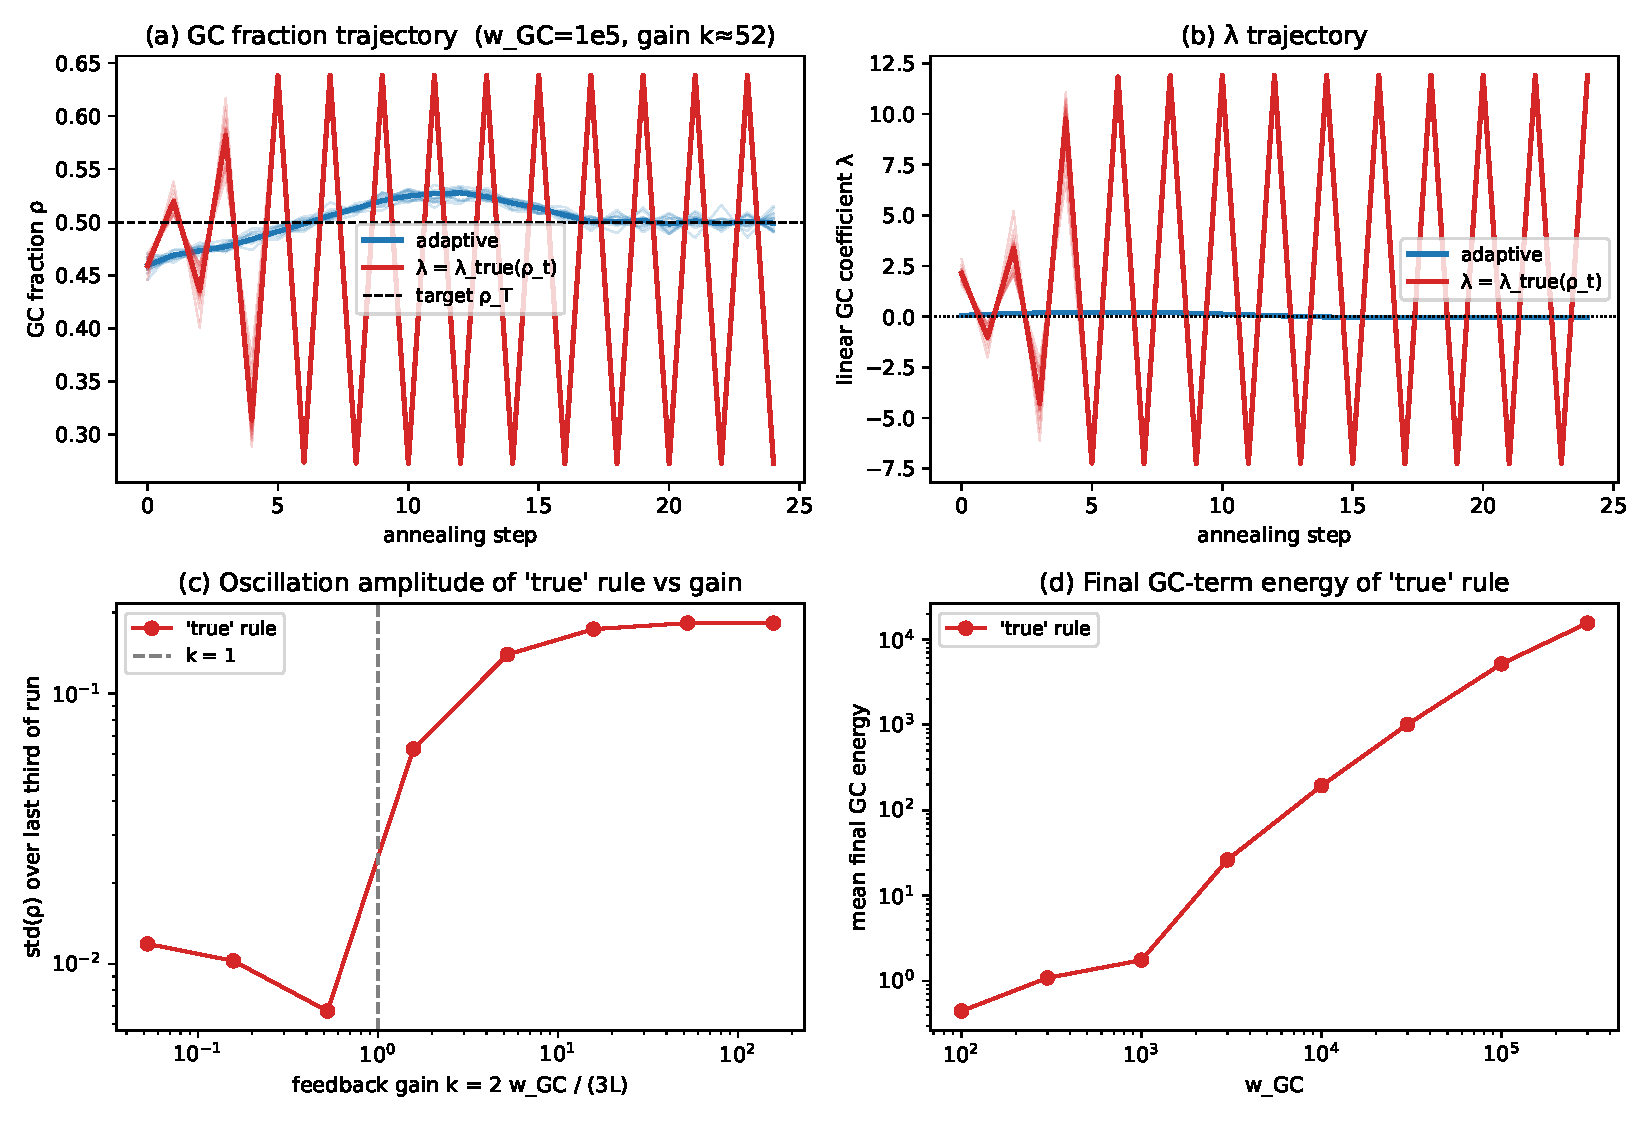
\includegraphics[width=0.95\textwidth]{images/gc_true_oscillation.pdf}
\caption{\textbf{The direct rule $\lambda = \lambda_{\mathrm{true}}(\rho_t)$ is unstable.}
\textbf{(a,b)}~GC fraction $\rho$ and linear coefficient $\lambda$ across annealing steps on the spike protein, $w_{\mathrm{GC}} = 10^5$ (hard setting).
Light traces: 16 individual chains. Bold: mean over chains.
The adaptive rule (blue) quickly settles to $\rho \approx \rho_T = 0.5$ with $\lambda \approx {-}0.05$; the direct rule (red) locks into a period-2 limit cycle with $\rho$ alternating between $0.27$ and $0.64$ and $\lambda$ alternating between $+11.9$ and $-7.3$ every single step.
\textbf{(c,d)}~Sweep of $w_{\mathrm{GC}}$ for the direct rule. Oscillation amplitude (std of $\rho$ across the last third of the run) is noise-level below the predicted threshold $k = 2 w_{\mathrm{GC}} / (3L) = 1$ (dashed line) and saturates at the sampler's physical response range ($\approx 0.18$) well above it. The final GC-term energy grows by orders of magnitude across the same sweep.}
\label{fig:gc-osc}
\end{figure}

\paragraph{Linear stability analysis.}
The direct rule is a pure proportional feedback controller:
\begin{equation}\label{eq:direct-rule}
  \lambda_{t+1} \;=\; -k\,(\rho_t - \rho_T),
  \qquad
  k \;\mathrel{:=}\; \frac{2\,w_{\mathrm{GC}}}{3L}.
\end{equation}
The loop is closed by the sampler: given enough Gibbs sweeps at inverse temperature $\beta_t$, the new bias $\lambda_{t+1}$ drives the chain to a new equilibrium GC fraction $\rho_{t+1}$.
For a single categorical position $c_p$ whose Gibbs distribution is $\propto \exp(\beta(h_p(k) + \lambda\, g(c_p^{(k)})))$ (THRML's weight convention), the standard exponential-family identity gives
$\partial\langle g(c_p)\rangle/\partial\lambda = \beta \,\mathrm{Var}_p(g)$, and summing over positions yields the per-chain susceptibility
\begin{equation}\label{eq:susceptibility}
  \frac{\partial \rho}{\partial \lambda}\bigg|_{\lambda=0}
  \;=\; \frac{\beta_t}{3L}\sum_{p=1}^{L} \mathrm{Var}_p\!\big(g(c_p)\big)
  \;=:\; \chi(\beta_t).
\end{equation}
Linearising \cref{eq:direct-rule} together with the sampler response around $\rho_T$ gives
\begin{equation}\label{eq:linear-loop}
  \rho_{t+1} - \rho_T \;\approx\; -A(\beta_t)\,(\rho_t - \rho_T),
  \qquad
  A(\beta_t) \;=\; k\cdot \chi(\beta_t).
\end{equation}
The fixed point $\rho = \rho_T$ is stable iff $|A| < 1$ and unstable otherwise; the sign of $A$ is always positive, so as soon as $A > 1$ the iteration produces a growing two-sided overshoot, i.e.\ a geometrically expanding 2-cycle.

For the codon problem on \emph{E.\ coli}-weighted tables, the per-position variance of the GC count $\mathrm{Var}_p(g)$ averages to $\mathcal O(0.3)$ at moderate $\beta_t$, giving $\chi(\beta_t) \sim 0.1\,\beta_t$ as an order-of-magnitude estimate (the true $\chi$ grows sublinearly at large $\beta_t$ because the per-position distribution concentrates on the locally-favoured codon and its variance decreases).
To leading order,
\begin{equation}\label{eq:A-estimate}
  A(\beta_t) \;\sim\; 0.1\,\beta_t \cdot \frac{2 w_{\mathrm{GC}}}{3L}.
\end{equation}
The annealing schedule spans $\beta_t \in [0.3, 100]$.
At the hard-weight setting $w_{\mathrm{GC}} = 10^5$ ($k \approx 52$), this estimate gives $A$ in the range $\approx 1.6$ to $\approx 520$ -- unstable from the very first step.
At the standard Fox weights $w_{\mathrm{GC}} = 1$ ($k \approx 5\!\times\!10^{-4}$), $A$ never exceeds $\approx 5\!\times\!10^{-3}$, and the direct rule would in fact work there.
The oscillation only arises in regimes where the GC term is heavily enforced -- which is precisely the regime in which any GC correction is needed at all, and in particular the hard-weight setting used for the stress tests in the main text.

\paragraph{Threshold verified by sweep.}
\Cref{fig:gc-osc}c,d sweeps $w_{\mathrm{GC}}$ through two-and-a-half orders of magnitude for the direct rule.
The transition between the stable and oscillating regimes occurs sharply at $k \approx 1$ (between $w_{\mathrm{GC}} = 10^3$ and $3\!\times\!10^3$), as predicted by \cref{eq:linear-loop}. Above that threshold the amplitude grows until it saturates at $\approx 0.18$: with a bias of magnitude $|\beta \lambda| \gg 1$, the sampler pushes every position to its lowest- or highest-GC codon, and the feasible range of $\rho$ over the codon table is the physical ceiling on the 2-cycle's amplitude.

\paragraph{Why the adaptive rule is stable.}
Replacing \cref{eq:direct-rule} with the integral rule of \cref{eq:lambda-update} gives a two-dimensional linear map in $(\rho - \rho_T,\,\lambda)$ whose Jacobian has eigenvalues $\{0,\;1 - \eta\,\chi(\beta_t)\}$.
The fixed point is stable whenever $\eta\,\chi(\beta_t) \in (0, 2)$.
Crucially, this closed-loop gain is $\eta\,\chi$, \emph{independent of} $w_{\mathrm{GC}}$: the integrator decouples the per-step feedback gain from the strength of the quadratic penalty it is emulating.
Since $\chi(\beta_t)$ is an $\mathcal O(1)$ quantity bounded over the entire annealing schedule -- at small $\beta_t$ it scales linearly with slope ${\sim}0.1$ (the average codon-table GC variance divided by three), at large $\beta_t$ it decays back toward $0$ as each position's distribution concentrates on the locally-favoured codon -- a choice of $\eta = \mathcal O(1)$ keeps $\eta\chi$ safely inside $(0, 2)$ for \emph{any} $w_{\mathrm{GC}}$. Our production values ($\eta = 1.0$ for Potts and $\eta = 0.9$ for Ising; \cref{tab:potts-params,tab:ising-params}) sit comfortably in this range.

The clamp of \cref{eq:clip} plays a secondary but important role: the integrator, left alone, could accumulate $\lambda$ past $\lambda_{\mathrm{true}}$ at large $\beta_t$.
At that point the linear surrogate would be \emph{stronger} than the quadratic term it is replacing, and its competition with the codon-usage and repeat terms would distort the objective.
The clamp to $\lambda_{\mathrm{true}}(\rho_t)$ is the natural upper bound: once $\lambda$ reaches $\lambda_{\mathrm{true}}$, the linear approximation is already as strong as the true quadratic gradient at the current $\rho_t$, and further integration would over-penalise GC deviation.

In short, the right way to use $\lambda_{\mathrm{true}}$ is as a \emph{bound}, not as a \emph{target}: the adaptive rule walks monotonically toward $\lambda_{\mathrm{true}}$ from the previous value via small integrator steps, while the direct rule jumps to $\lambda_{\mathrm{true}}$ every step -- and, because the sampler's response gain $\chi$ is large enough to make $k\chi > 1$ at interesting weights, those jumps do not damp out but lock into a 2-cycle instead.

\subsection*{Integration with annealing and flash-sample-read}

Because $\lambda$ enters the Potts bias linearly, it is scaled by the current inverse temperature $\beta_t$ before being compiled into the model. The model biases at step~$t$ become
\begin{equation}\label{eq:compiled-bias}
  \tilde h_p^{(t)}(k) \;=\; \beta_t \,\Big(\, h_p(k) + \lambda_t \, g\!\left(c_p^{(k)}\right)\,\Big).
\end{equation}
In the Ising case, $\tilde h_p^{(t)}$ is subsequently compiled to Ising biases via domain-wall encoding (Supplementary Note~1, \cref{eq:bias,eq:bias-pairwise}).
The host algorithm at each annealing step is therefore:
\begin{enumerate}
  \item Read back the state of every chain from the TSU (or its simulator) and compute $\rho_t$ per chain.
  \item Update $\lambda_t \to \lambda_{t+1}$ via \cref{eq:clip}.
  \item Combine the new $\lambda_{t+1}$ with the scheduled $\beta_{t+1}$ (and, in the Ising case, $P_{t+1}$) to produce the biases of \cref{eq:compiled-bias}.
  \item Flash the new weights to the TSU and run \texttt{steps\_per\_beta} Gibbs sweeps.
\end{enumerate}
The cost on a real TSU is \emph{zero} additional flashes: weights would have to be re-flashed every annealing step anyway in order to update $\beta_t$ (and $P_t$ in the Ising case), so folding the updated $\lambda_{t+1}$ into the same flash adds no new operations.
The additional host work consists only of one reduction per chain (to compute $\rho_t$) and a handful of scalar operations.

\subsection*{GC-sorted codon ordering}

In the Ising / domain-wall formulation, a single spin flip moves the underlying Potts variable between two \emph{adjacent} indices, $k \leftrightarrow k{\pm}1$ (see Section~4.4 of the main text).
For the linear GC bias in \cref{eq:lambda-bias} to actually guide the domain wall, the codon indices at each position must be arranged so that adjacent indices differ by as little as possible in GC count.
Otherwise, moving the domain wall by one spin would cause discontinuous jumps in GC content, which the linear approximation cannot compensate for smoothly.

We therefore order the codons at each position by ascending GC count, with alphabetical tiebreaking among codons of equal GC count.
This is the ordering returned by \texttt{SORTED\_CODON\_TABLE} in \path{codons/problem.py}, and it is used in both the Potts and Ising formulations (the Potts chain does not require it, but using the same ordering keeps weight computation consistent between the two models).
\Cref{tab:codon-ordering} shows the resulting ordering for three representative amino acids.

\begin{table}[H]
\centering
\caption{GC-sorted codon ordering for representative amino acids. Index 0 is the lowest-GC codon; adjacent indices differ by at most 1 in GC count. The number in parentheses is the GC count of each codon.}
\label{tab:codon-ordering}
\vspace{2mm}
\begin{tabular}{llccccccl}
\toprule
Amino acid & \#Codons & Idx 0 & Idx 1 & Idx 2 & Idx 3 & Idx 4 & Idx 5 & DW spins \\
\midrule
Leucine (L) & 6 & TTA (0) & CTA (1) & CTT (1) & TTG (1) & CTC (2) & CTG (2) & 5 \\
Alanine (A) & 4 & GCA (2) & GCT (2) & GCC (3) & GCG (3) & -- & -- & 3 \\
Phenylalanine (F) & 2 & TTT (0) & TTC (1) & -- & -- & -- & -- & 1 \\
\bottomrule
\end{tabular}
\end{table}

\noindent
Under this ordering every single spin flip changes the GC content of the sequence by at most 1, and flips between codons of equal GC count are GC-neutral.
Two consequences follow.
First, the GC landscape seen by the domain wall becomes locally smooth: the term $\lambda \cdot g(c_p^{(k)})$ is monotone (up to ties) in the Potts index $k$, so after conversion to Ising biases via first differences (\cref{eq:bias}) the linear GC coefficient produces a spatially uniform shift along each spin chain rather than a sign-alternating pattern.
Second, the adaptive scheme of \cref{eq:clip} acquires a natural interpretation in spin space: $\lambda$ is a single scalar knob that uniformly shifts the bias along every domain wall, continuously trading off the cost of moving the wall one step inward against the benefit (or cost) of gaining one unit of GC.
An arbitrary codon ordering would scramble this relationship and require a per-codon schedule to achieve the same effect, which is incompatible with a single global $\lambda$.

% ============================================================
% REFERENCES
% ============================================================
\bibliography{refs}

\end{document}
